\chapter{Fejlesztői dokumentáció} % Developer guide
\label{ch:impl}

\section{Tervezés}

\subsection{Kezdeti tervek}
Mivel egy játék (legyen akármekkora is) egy bonyolult rendszer, és mivel alapértelmezetten is egy jó gyakorlat, a projekt elejétől kezdve meg szerettem volna tervezni, átfogóalga a különböző rendszereket. Tudtam előre, hogy a Unity játékmotort fogom használni a példajáték elkészítéséhez, és a tervminták alkalmazására és fontosságára Jason Weimann\cite{jason}, DapperDino\cite{dapperDino} és a Game Programming Patterns-ben\cite{gameProgrammingPatterns} olvasottak inspiráltak. Azt is figyelmemben tartottam, hogy szakdolgozatom célja a tervezési minták és programozási elvek felhasználása a játékfejlesztésben és nem feltétlenül egy teljes mértékben kidolgozott játék piacra dobása.\\*
Mindezek után három dolgot tartottam fontosnak eleinte, a játékos (és ellenségek) statemachine-ját, egy általánost leírás az alap rendszerek kapcsolatáról, valamint a játékom elkészítése a S.O.L.I.D elvek szerint.
\begin{figure}[H]
	\noindent\makebox[\textwidth]{
	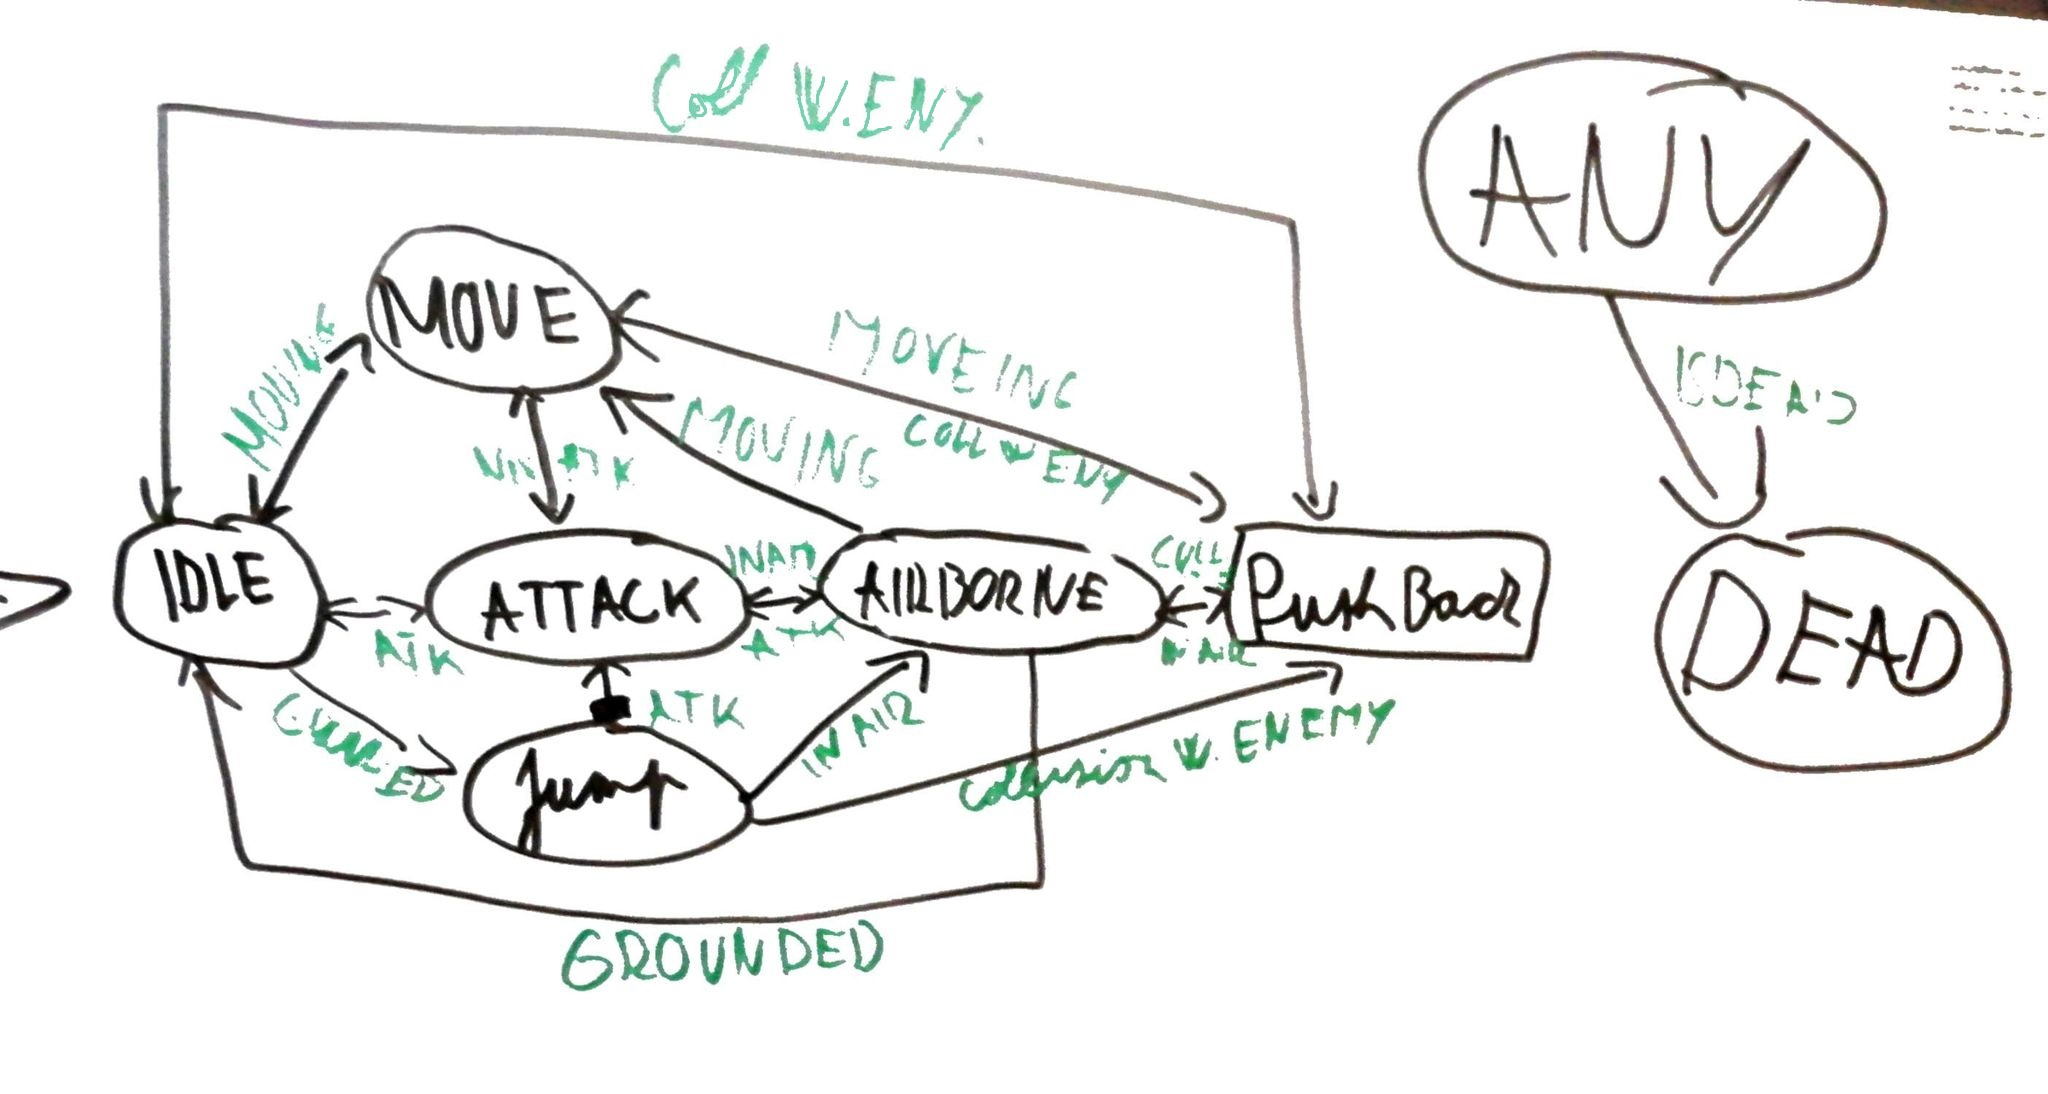
\includegraphics[width= 0.8\textwidth]{statemachine}}
	\caption{Kezdeti statemachine}
	\label{statemachine}
\end{figure}

\begin{figure}[H]
	\noindent\makebox[\textwidth]{
	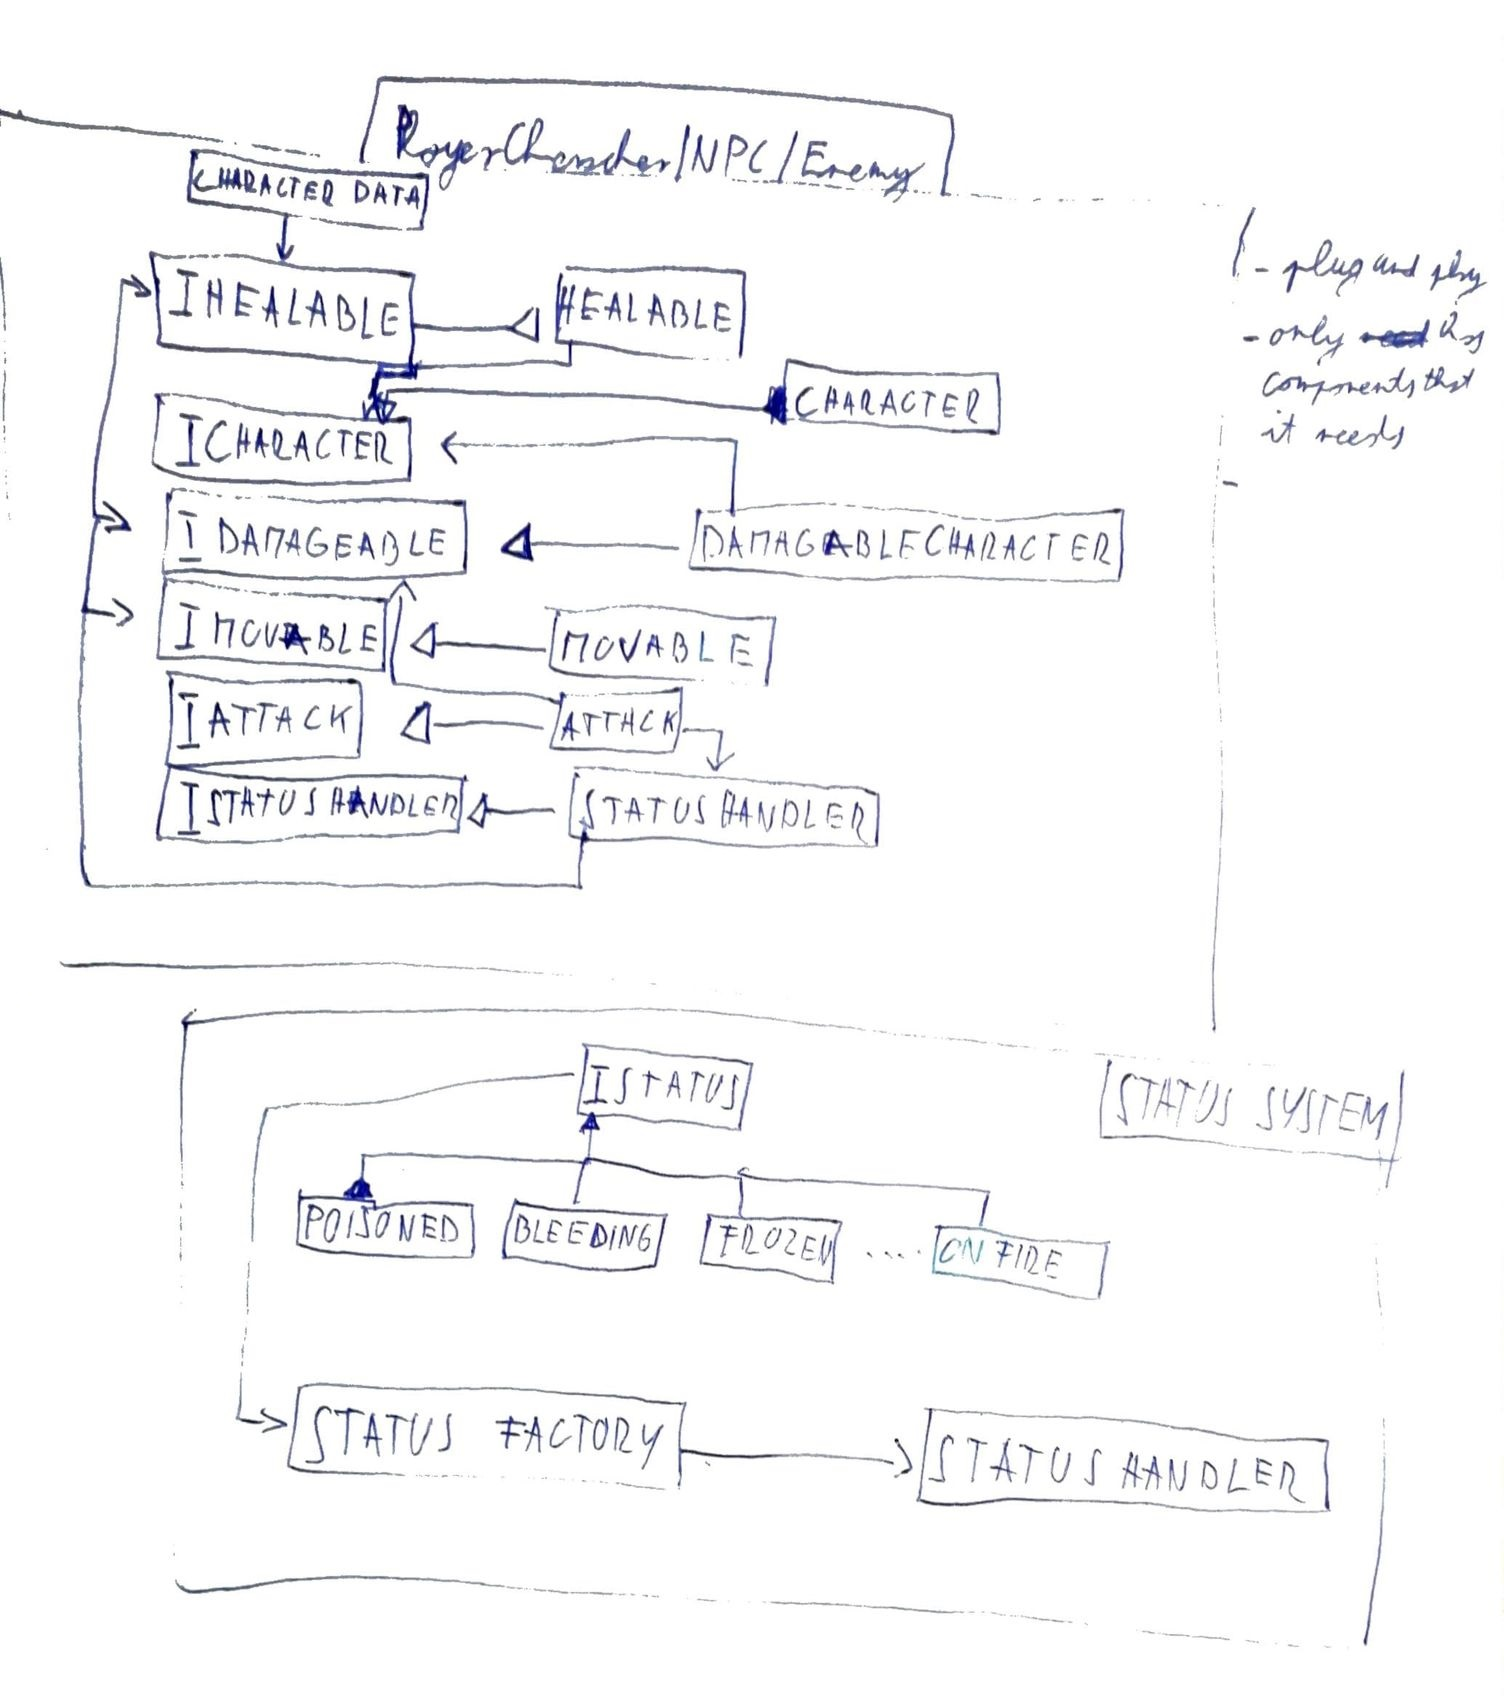
\includegraphics[width= 0.8\textwidth]{statussys}}
	\caption{Rendszerek általános leírása}
	\label{statussys}
\end{figure}

Azonban hamar rájöttem, hogy bizonyos bonyolultan rendszerek kapcsolatát érdemes jobban kifejteni. Ilyen volt a támadással foglalkozó csoport is, ahol három kisebb rendszer összeépítését kellett kivitelezni. Ezek a varázslatok, státuszeffektusok és maga a támadás rendszere voltak.

\begin{figure}[H]
	\noindent\makebox[\textwidth]{
	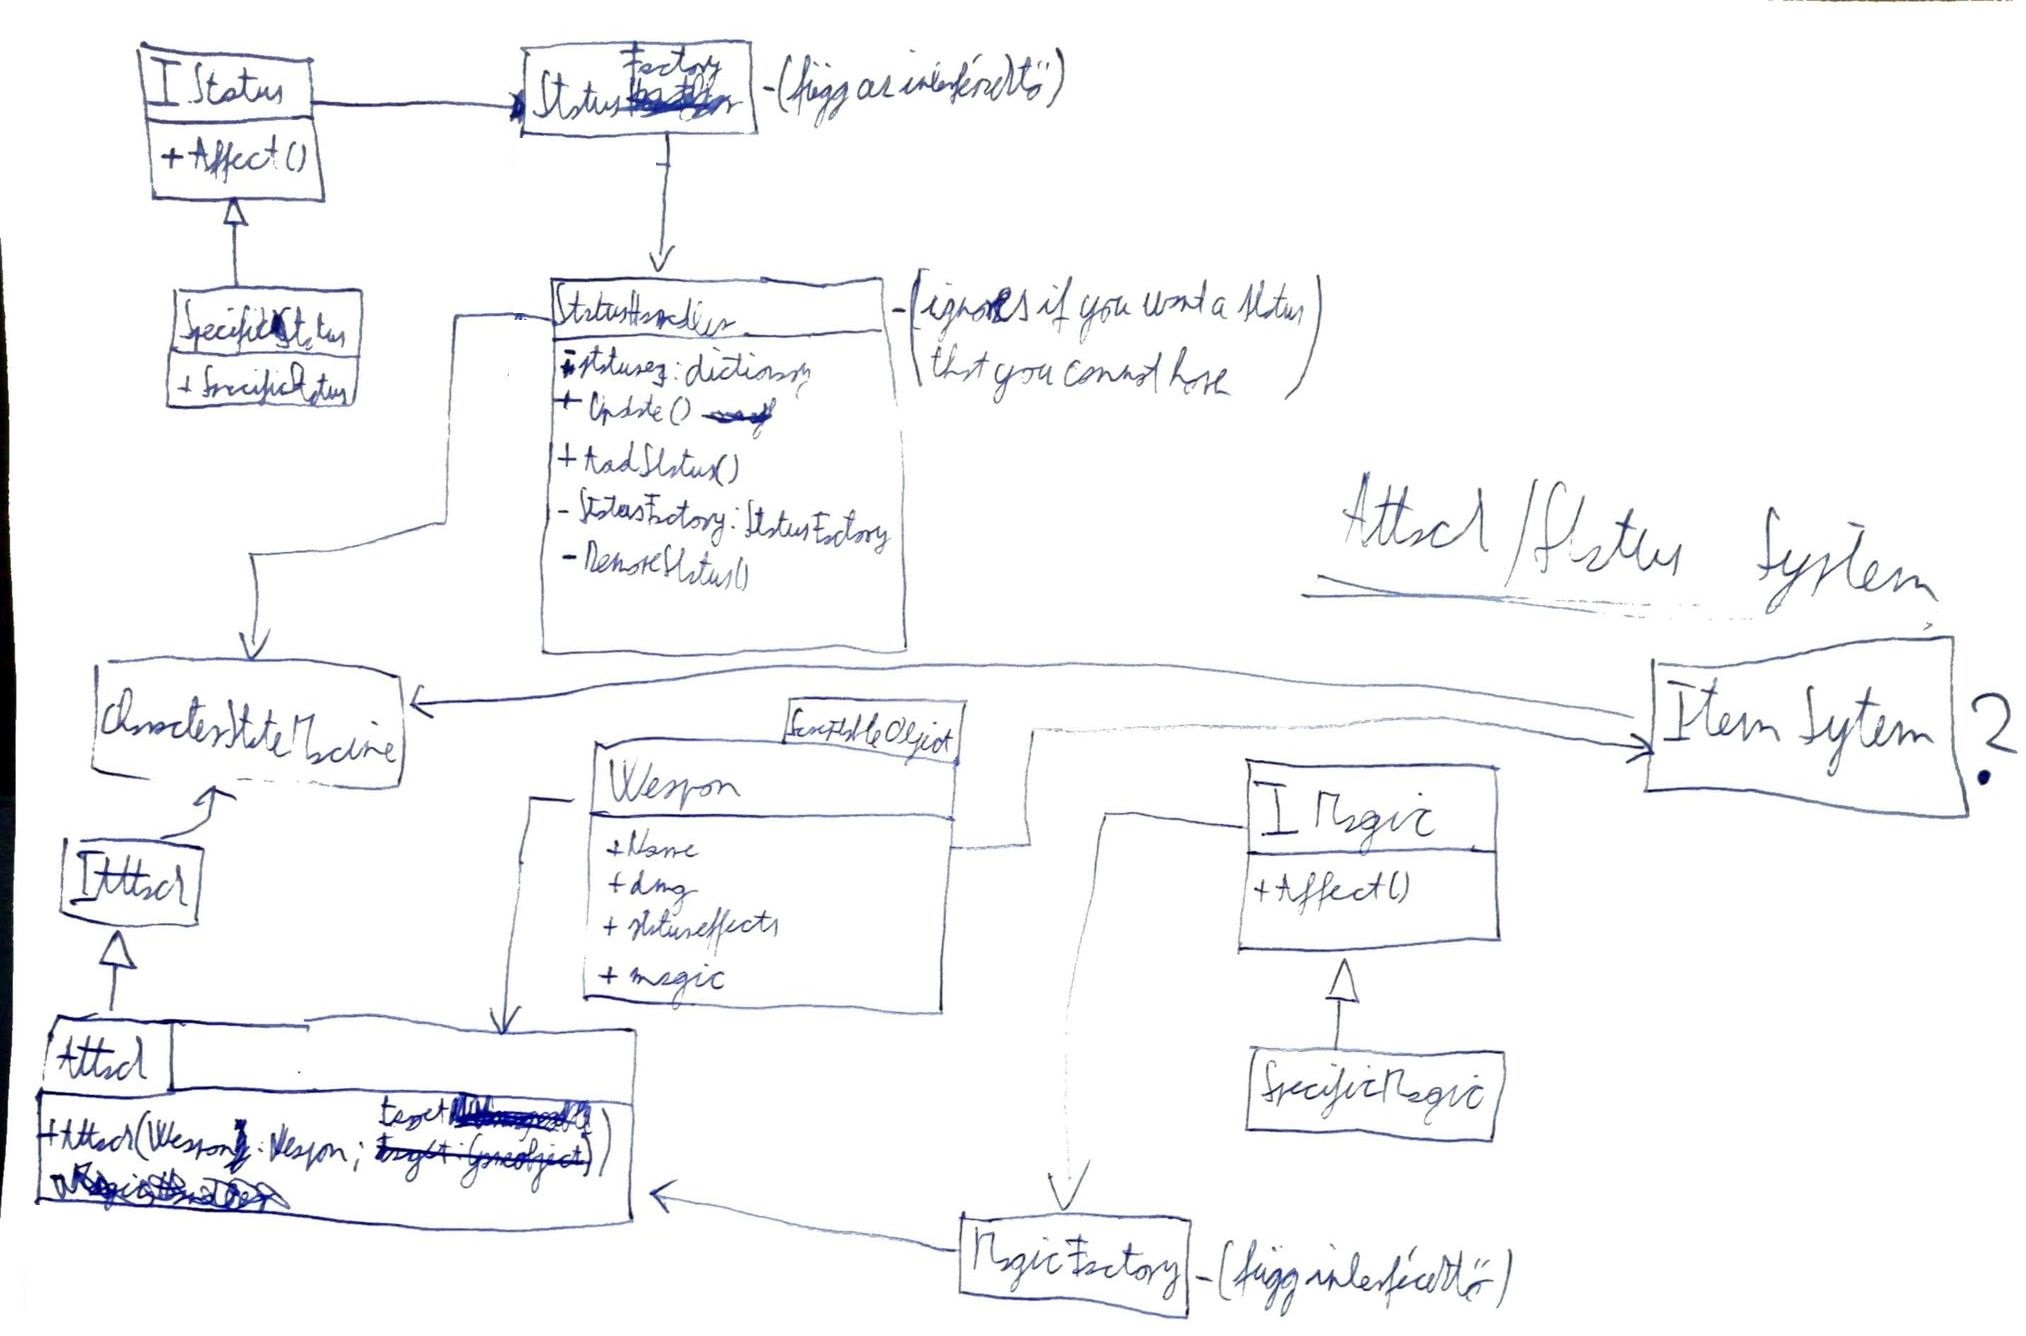
\includegraphics[width= 1\textwidth]{all}}
	\caption{Támadási rendszer}
	\label{all}
\end{figure}

\subsection{Unity}
A Unity játékmotor egy cross-platform komponens alapú játékfejlesztői motor. Ebben a fejlesztői környezetben, relatívan egyszerűen hozhatunk létre játékokat (főleg az új visual scripting segítségével, hiszen így fejlesztők nem kényszerülnek rá a C\# nyelv elsajátítására). Unity-ben 2 fontos dolgot kell megértenünk, egyik az Editor, amit használni fogunk a színterünk komponálására, valamit a komponenseink (GameObjects) létrehozására, a másik a monoBehaviour-ök megértés, hiszen ez az osztály az összes Unity script ősosztálya.\\
Először is a \textbf{Unity Editor}-ról beszélnék. Ez a Unity Engine gafikus interfésze, innen érhetjük el a Unity által biztosított funkciókat, mint például az \textit{animator}, ahol animációk átmeneteit határozhatjuk meg, a \textit{shader graph}-ot, ahol egy grafikus felületen készíthetünk vertex és fragment shader-eket, vagy akár a \textit{test runner}-t, hogy párat említsek.\\*
Azonban a 2 legfontosabb funkciója az Editornak a színtereink(scenes) és \textit{gameObject}-jeink komponálása. A színtereinken készíthetünk pályákat, menüket, adhatunk hozzá hangforrásokat, fényeget vagy utóhatások, nem mellesleg ide kell hozzáadnuk a gameObject-eket, hogy megjelenjenek.\\*
A \textit{gameObject}-ekteket el lehet képzelni úgy, mint egy üres dobozt,amihez különböző komponenseket adhatunk. Ha azt akarjuk, hogy ne láthatatlan legyen a dobozunk adhatunk hozzá egy \textit{Sprite Renderer}-t, ha akarjuk, hogy a fizika hasson rá akkor hozzáadhatjuk a \textit{Rigidbody} komponenst és így tovább. Egy gameObject rengeteg minden lehet és több funkciót is elláthat, nem mellesleg rájuk aggathatjuk a saját script-jeinket is hogy valami egyedi hatást/viselkedést érjünk el.\\
Most hogy beszéltem az Editor-ról, a helyről, ahol a játék építése folyik beszélnék egy kicsit az egyik legfontosabb építőelemről, a \textbf{monoBehaviour}-ről, ami az összes script-ünk ősosztálya, amit egy \textit{gameObject}-re rá akarunk rakni, mint egy komponenst. A monoBehaviour és minden leszármazottja egy olyan osztály, amit nem lehet a \textbf{new} kulcsszóval példányosítani, csak az \textit{addComponent} függvénnyel. Ebből következve ezen osztályok, csak egy \textit{gameObject}-en élhetnek és kötöttek annak élettartalmához.\\*
A monoBehaviour biztosít számunkra pár fontos metódust is \cite{unityDocs}.
\begin{itemize}
	\item \textbf{Start} - inicializációs fázis utolsó lépése.
	\item \textbf{FixedUpdate} - fizikai frissítés. Itt lehet olyan fizikai számításokat kezelni, amiket minden ütemezett fizikai frissítésben végre akarunk hajtani.
	\item \textbf{OnCollisionXXX} - mi történjen ha valami ütközés történik.
	\item \textbf{Update} - elépzelhető mint egy monoBehaviour-re korlátozott \textit{gameLoop}. Akkor használjuk, ha ismétlődő számításokat akarunk végrehajtani (minden frame-ben).
\end{itemize}

\begin{figure}[H]
	\noindent\makebox[\textwidth]{
	\includegraphics[width= 1\textwidth]{thdfT}}
	\caption{MonoBehaviour életciklusa}
	\label{thdfT}
\end{figure}

\subsection{S.O.L.I.D.}
A S.O.L.I.D. elvek\cite{solid}

\textbf{S - Single-responsiblity Principle}, avagy az \textit{Egyetlen felelősség elve}\\
Ennek az elvnek a lényege, hogy egy osztálynak, egyetlen egy oka lehet a változásra, vagyis egy céljának kell lennie. Ennek az elvnek a megvalósítása Unity-ben triviális, hiszen kisebb odafigyeléssel ez adódik is a komponens alapú összetételből.

\textbf{O - Open-closed Principle}, avagy az \textit{Nyílt/zárt elv}\\
Itt a legfontosabb tudnivaló, hogy egy objektumnak képesnek (nyitottnak) kell lennie a bővítésekre, azonban ezeknek a bővítéseknek nem szabad módosítania a meglévő osztályt, zárva kell lennie a módosításokra tekintve. Ugye ez az elv interfészek és ősosztályok megvalósításával könnyen elérhető, hiszen ha megvannak a mintáink, hogy miképp kell egy osztálynak felépülnie, és azt meg is valósítottuk, esetleg egységtesztekkel le is védtük működését, akkor annak módosítása hiba nélkül nehéz lesz, azonban a bővítése triviális. Az a fontos itt, hogy a régi kódban lévő logika a bővítés miatt ne kényszerüljön az új kódrész függésére, ebben az esetben lehet érdemes meggondolni a kód faledarabolását a \textit{Egyetlen felelősség elve} mintájára.

\textbf{L - Liskov Substitution Principle}, avagy az \textit{Liskov helyettesítési elv}\\
Liskov helyettesítési elv lényege, hogy minden osztályt be kéne tudni helyettesíteni annak ősosztályába, interfészébe. Ez egy rendkívül fontos megállapítás, hiszen ezzel meg tudjuk szüntetni a függést egy specifikus osztályimplementációtól, ezáltal képesek leszünk könnyen cserélni konkrét működést egy komponensben/osztályban annak megváltoztatása nélkül.

\textbf{I - Interface Segregation Principle}, avagy az \textit{Interfész elválasztási elv}\\
Az elv azt mondja ki, hogy egy osztálynak nem szabad függenie olyan interfészektől, függvényektől, amiket nem valósít meg, nem használ. Ez könnyen felfogható, úgy mint az \textit{Egyetlen felelősség elve} alkalmazása interfészekre, hiszen így több kisebb közelebb kapcsolódó interfészt kapunk, amiket szabadon implementálhat egy osztály szükség szerűen, ellentétben egy nagy interfésszel.

\textbf{D - Dependency Inversion Principle}, avagy az \textit{Függőség megfordítási elv}\\
Ez az elv azt mondja ki, hogy az entitásoknak absztrakciókon kell függeniük, valamint, hogy magasabb rendű rendszereknek nem szabad függeniük az alacsonyrendűektől. Ezt a komponens alapú Unity-ben könnyen elérhetjük, hiszen ha osztályain egy interfészt implementálnak, ami megfelel az absztrakciónak és ezen osztályainkat a \textit{Liskov helyettesítési elv} és a \textit{Egyetlen felelősség elve} szerint hoztuk létre és mint Unity-s komponens használunk, akkor a magas szintű rendszereink tudnak csak az absztrakciótól függeni és Unity-ben intuitívan megvalósulni.

Mindezeket látva a Unity mint keretrendszer rendkívül alkalmas a S.O.L.I.D. elvek alkalmazására.

\subsection{Tervminták}
Miután átnéztük, hogy milyen elvek szerint lett elkészítve a játék, térjünk is át a szakdolgozat lényegére, a felhasznált tervmintákra és azok hasznára szerepére. A Game Programming Patterns-ben\cite{gameProgrammingPatterns} olvasott tervmintákat, néhány más hasznos mintával kiegészítve fogom kifejteni itt részletesebben, Jason Weimann\cite{jason} és DapperDino\cite{dapperDino} implementációit és példáit alapul véve. Ezek a minták kettő csoportba sorolhatók alapvetően, amik az \textbf{általunk implementált} tervezési minták és a \textbf{Unity/C\# által biztosított} tervezési minták, kezdjük is az utóbbikkal.

\textbf{Game Loop} - avagy a \textit{Játékciklus}\\
Ez a játék magja, legfontosabb alapköve. A Unity automatikusan biztosítja, nincs szükség egy komponáló osztályra, ahol egy while ciklusban hívódnának osztályaink. A tervminta lényeg, hogy biztosítanunk kell egy a játék terminállásáig tartó folyamatos környezetet, ahol a játékos inputot, eseményeket és a játékon belüli időt kezelünk kell. Mivel ezt a modern játékfejlesztői környezetek alapértelmezetten tudják és elrejtik a felhasználó elöl (,mint a Unity), ezért érdemes úgy tekinteni az ezen eszközökkel történő fejlesztés közben, mintha mindig a Játékciklusban lennénk.

\textbf{Update Method} - avagy a \textit{Frissítési metódus}\\
Ez a minta mögött az a gondolat húzódik, hogy vannak bizonyos számítások (például egy karakter pozícióváltozásából származó újrarajzolás) amiket minden egyes kirajzolt frame-ben végre szeretnénk hajtani. Unity-ben ezt a tervmintát még jobban felaprították, hiszen a monoBehaviour biztosít számunkra három különböző Update metódust is. A monoBehaviour életciklusa szerint \textit{FixedUpdate} amiben a fizikai számítások hajtódnak végre fix intervallumonként, \textit{Update}, ami egy általános frissítési metódus, itt végezzük a saját logikánk módosításainak nagyját, legvégül a \textit{LateUpdate}, ami egy a sima Update metódust, animáció frisítéseket és a coroutine-okat követő frissítés, ahol olyan operációkat hajthatunk végre, amiket az Update után szeretnénk végrehajtani.

\textbf{Component} - avagy a \textit{Komponens}\\
Ez a tervminta egy csoportosítási problémát szándékozz megoldani hasonlóan a Egyetlen felelősség elvéhez. Ezt a Unity szintén alapjaiban támogatja, hiszen az egész játékmotor komponens alapú (rigidbody, amiator, spriteRenderer, mint külön komponensek amiket egy gameObject-re tudunk ráaggatni, mint a saját script-jeinket).

\textbf{Type Object/Flyweight} - avagy a \textit{Típusobjektum/Pehelysúlyú}\\
Ezen tervezési minták, habár különböző, azonban egymáshoz rendkívüli módon kapcsolódó koncepciókat írnak le. A Típusobjektum lényeg, hogy a példányspecifikus adatokat a típusolt objektumban tároljuk, míg az ezeket alkalmazó metódusokat/függvényeket, vagy közös adatokat a típusobjektumban definiáljuk, így a közös részeket és az egyedi adatokat elszeparáljuk. A Pehelysúlyú tervminta nagyon hasonlóan el akarja különíteni a példányspecifikus adatokat a megosztott minden azonos osztály számára szükséges és azonos adatoktól, ezáltal létrehozva egy pehelykönnyű osztályt. Mint láthattuk mindkettő tervminta célja a példányspecifikus adatok szeparálása, Unity-ben erre rendkívül jól használhatóak a \textit{ScriptableObject}-ek. Ezek egy különleges osztályok, amik többnyire adatstruktúrákat és közös működéseket írnak le. Miután definiáltunk egy ScriptableObject-et, azt legtöbbször nem a tradícionális módon kódból példányosítjuk, hanem a Unity Editor-ban hozzuk létre, mint új Asset-et, itt tudjuk az általunk megadott mezők értékeit kitölteni. Ha egy a ScriptableObject-et hozzárendelünk GameObject-ekhez akkor a különböző GameObject-ek között a ScriptableObject azonos marad, csak egyszer töltődik be a memóriába és minden változást az összes GameObject lát ha az adott ScriptableObject hozzá van rendelve.

\textbf{Observer} - avagy a \textit{Figyelő}\\
Ez a tervminta annyira elterjedt, hogy a C\# nyelvbe natívan támogatva is van az eseményrendszeren keresztül. Unity-ben is támogatva van a C\#-os eseményrendszer, azonban a Unity-biztosít egy saját eseménykezelést is ez nem más mint a \textit{Unity event}-ek. Ezek lényegében egy kényelmi funkciót látnak el, hogy égszerűen tudjunk az Editor-ban összekötni eseményeket, ezen események általában olyan elemek, amit kóddal ritkán váltunk ki (általában UI gombnyomások vagy az Input System-ből érkező események), azonban saját funkciót szeretnénk kötni különösebb komplikáció nélkül.


\cleardoublepage
\section{Megvalósítás}

\begin{figure}[H]
	\noindent\makebox[\textwidth]{
	\includegraphics[width= 1.1\textwidth]{GeneralComponentSystem}}
	\caption{Általános komponens kapcsolat}
	\label{GeneralComponentSystem}
\end{figure}

\subsection{Felhasználói esetek}
\begin{figure}[H]
	\noindent\makebox[\textwidth]{
	\includegraphics[width= 1.1\textwidth]{useCase}}
	\caption{Felhasználói eset diagram}
	\label{useCase}
\end{figure}

\subsection{Státusz rendszer}

\begin{figure}[H]
	\noindent\makebox[\textwidth]{
	\includegraphics[width= 1.1\textwidth]{StatusSystem}}
	\caption{Státusz rendszer UML}
	\label{StatusSystem}
\end{figure}

\subsection{Varázslás rendszer}

\begin{figure}[H]
	\noindent\makebox[\textwidth]{
	\includegraphics[width= 1\textwidth]{MagicSystem}}
	\caption{Varázslat rendszer UML}
	\label{MagicSystem}
\end{figure}

\subsection{Játékos rendszer}

\subsection{Ellenség rendszer}

\subsection{Adattárolás}

\subsection{GUI}

\subsection{Zene}

\subsection{Pályák felépítése}

\subsection{CI/CD pipeline}

\cleardoublepage
\section{Tesztelés}

\subsection{Egységtesztek}

\begin{figure}[H]
	\noindent\makebox[\textwidth]{
	\includegraphics[width= 0.5\textwidth]{tests}}
	\caption{Az egységtesztek eredményei}
	\label{tests}
\end{figure}

\begin{figure}[H]
	\noindent\makebox[\textwidth]{
	\includegraphics[width= 1\textwidth]{codeCoverage}}
	\caption{A Logic assembly tesztelési lefedettsége}
	\label{codeCoverage}
\end{figure}


\subsection{Kézi Tesztelés}

\subsection{Tesztelési konklúzió}